% Options for packages loaded elsewhere
\PassOptionsToPackage{unicode}{hyperref}
\PassOptionsToPackage{hyphens}{url}
\PassOptionsToPackage{dvipsnames,svgnames,x11names}{xcolor}
%
\documentclass[
  onecolumn]{report}

\usepackage{amsmath,amssymb}
\usepackage{lmodern}
\usepackage{iftex}
\ifPDFTeX
  \usepackage[T1]{fontenc}
  \usepackage[utf8]{inputenc}
  \usepackage{textcomp} % provide euro and other symbols
\else % if luatex or xetex
  \usepackage{unicode-math}
  \defaultfontfeatures{Scale=MatchLowercase}
  \defaultfontfeatures[\rmfamily]{Ligatures=TeX,Scale=1}
\fi
% Use upquote if available, for straight quotes in verbatim environments
\IfFileExists{upquote.sty}{\usepackage{upquote}}{}
\IfFileExists{microtype.sty}{% use microtype if available
  \usepackage[]{microtype}
  \UseMicrotypeSet[protrusion]{basicmath} % disable protrusion for tt fonts
}{}
\makeatletter
\@ifundefined{KOMAClassName}{% if non-KOMA class
  \IfFileExists{parskip.sty}{%
    \usepackage{parskip}
  }{% else
    \setlength{\parindent}{0pt}
    \setlength{\parskip}{6pt plus 2pt minus 1pt}}
}{% if KOMA class
  \KOMAoptions{parskip=half}}
\makeatother
\usepackage{xcolor}
\usepackage[top=30mm,left=20mm,heightrounded]{geometry}
\setlength{\emergencystretch}{3em} % prevent overfull lines
\setcounter{secnumdepth}{-\maxdimen} % remove section numbering
% Make \paragraph and \subparagraph free-standing
\ifx\paragraph\undefined\else
  \let\oldparagraph\paragraph
  \renewcommand{\paragraph}[1]{\oldparagraph{#1}\mbox{}}
\fi
\ifx\subparagraph\undefined\else
  \let\oldsubparagraph\subparagraph
  \renewcommand{\subparagraph}[1]{\oldsubparagraph{#1}\mbox{}}
\fi


\providecommand{\tightlist}{%
  \setlength{\itemsep}{0pt}\setlength{\parskip}{0pt}}\usepackage{longtable,booktabs,array}
\usepackage{calc} % for calculating minipage widths
% Correct order of tables after \paragraph or \subparagraph
\usepackage{etoolbox}
\makeatletter
\patchcmd\longtable{\par}{\if@noskipsec\mbox{}\fi\par}{}{}
\makeatother
% Allow footnotes in longtable head/foot
\IfFileExists{footnotehyper.sty}{\usepackage{footnotehyper}}{\usepackage{footnote}}
\makesavenoteenv{longtable}
\usepackage{graphicx}
\makeatletter
\def\maxwidth{\ifdim\Gin@nat@width>\linewidth\linewidth\else\Gin@nat@width\fi}
\def\maxheight{\ifdim\Gin@nat@height>\textheight\textheight\else\Gin@nat@height\fi}
\makeatother
% Scale images if necessary, so that they will not overflow the page
% margins by default, and it is still possible to overwrite the defaults
% using explicit options in \includegraphics[width, height, ...]{}
\setkeys{Gin}{width=\maxwidth,height=\maxheight,keepaspectratio}
% Set default figure placement to htbp
\makeatletter
\def\fps@figure{htbp}
\makeatother

\makeatletter
\makeatother
\makeatletter
\makeatother
\makeatletter
\@ifpackageloaded{caption}{}{\usepackage{caption}}
\AtBeginDocument{%
\ifdefined\contentsname
  \renewcommand*\contentsname{Indice del contenuto}
\else
  \newcommand\contentsname{Indice del contenuto}
\fi
\ifdefined\listfigurename
  \renewcommand*\listfigurename{Elenco delle Figure}
\else
  \newcommand\listfigurename{Elenco delle Figure}
\fi
\ifdefined\listtablename
  \renewcommand*\listtablename{Elenco delle Tabelle}
\else
  \newcommand\listtablename{Elenco delle Tabelle}
\fi
\ifdefined\figurename
  \renewcommand*\figurename{Figura}
\else
  \newcommand\figurename{Figura}
\fi
\ifdefined\tablename
  \renewcommand*\tablename{Tabella}
\else
  \newcommand\tablename{Tabella}
\fi
}
\@ifpackageloaded{float}{}{\usepackage{float}}
\floatstyle{ruled}
\@ifundefined{c@chapter}{\newfloat{codelisting}{h}{lop}}{\newfloat{codelisting}{h}{lop}[chapter]}
\floatname{codelisting}{Lista}
\newcommand*\listoflistings{\listof{codelisting}{Elenco degli Elenchi}}
\makeatother
\makeatletter
\@ifpackageloaded{caption}{}{\usepackage{caption}}
\@ifpackageloaded{subcaption}{}{\usepackage{subcaption}}
\makeatother
\makeatletter
\@ifpackageloaded{tcolorbox}{}{\usepackage[many]{tcolorbox}}
\makeatother
\makeatletter
\@ifundefined{shadecolor}{\definecolor{shadecolor}{rgb}{.97, .97, .97}}
\makeatother
\makeatletter
\makeatother
\ifLuaTeX
\usepackage[bidi=basic]{babel}
\else
\usepackage[bidi=default]{babel}
\fi
\babelprovide[main,import]{italian}
% get rid of language-specific shorthands (see #6817):
\let\LanguageShortHands\languageshorthands
\def\languageshorthands#1{}
\ifLuaTeX
  \usepackage{selnolig}  % disable illegal ligatures
\fi
\IfFileExists{bookmark.sty}{\usepackage{bookmark}}{\usepackage{hyperref}}
\IfFileExists{xurl.sty}{\usepackage{xurl}}{} % add URL line breaks if available
\urlstyle{same} % disable monospaced font for URLs
\hypersetup{
  pdfauthor={Matteo Pedani},
  pdflang={it},
  colorlinks=true,
  linkcolor={blue},
  filecolor={Maroon},
  citecolor={Blue},
  urlcolor={Blue},
  pdfcreator={LaTeX via pandoc}}

\author{Matteo Pedani}
\date{}

\begin{document}
\ifdefined\Shaded\renewenvironment{Shaded}{\begin{tcolorbox}[boxrule=0pt, borderline west={3pt}{0pt}{shadecolor}, sharp corners, breakable, interior hidden, enhanced, frame hidden]}{\end{tcolorbox}}\fi

\listoffigures
\listoftables
\textbf{Gentile Dott.ssa Maura Baroli,}

È Da parecchio tempo che lavoro a questo ambizioso progetto che ti
sottopongo, che come la tela di Penelope è stato costruito e disfatto
più e più volte.

Quando sono venuto a fare il sopralluogo in Sardegna da lì a poco
sarebbe iniziato il covid cioè un paio anni fa, ma per me è come se
fossero passati decenni, la mia vita è completamente cambiata, ponendomi
davanti a difficili e tragici cambiamenti.

Non ultima la difficoltà di trovare il necessario supporto economico.
Finalmente poco tempo fà abbiamo creato una startup la ``Nocerosso
s.r.l.'' che ha come obbiettivo la ricerca e sviluppo nel settore
marino.

Non vedo l'ora di venire a parlarti ed iniziare a lavorare.

Ringraziandoti per l'attenzione, resto a disposizione per qualsiasi
ulteriore informazione.

Cordiali saluti,

Dato che ho messo un paio di grafici qui può leggere la
\href{https://nocerosso.com/lettera.html}{lettera.html} completa oppure
stamparla \href{https://nocerosso.com/lettera.pdf}{lettera.pdf}

\textbf{Matteo Pedani}

\newpage

\hypertarget{business-plan}{%
\subsection{Business Plan}\label{business-plan}}

Sono lieto di presentare un Business Plan innovativo e ambizioso, che
punta a sviluppare una tecnologia all'avanguardia per la produzione di
energia elettrica dalle onde del mare, e dal sole.

Si tratta di un sistema integrato per la allevamento ittico in alto mare
e di ostriche nelle lagune di Oristano prevede l'impiego di campi di boe
``point absorber'' e pannelli fotovoltaici galleggianti per la
produzione di energia elettrica. L'utilizzo congiunto di tali
tecnologie, insieme all'allevamento ittico e alle ostriche, comporta
numerosi vantaggi.

Uno dei maggiori vantaggi di questo sistema integrato è l'impiego
cointemporaneo della stessa manodopera per il controllo dei campi di boe
e pannelli solari e per l'allevamento ittico e delle ostriche, che porta
ad un aumento della resa per unità lavorativa. Ciò significa che i
lavoratori possono controllare sia le attività di coltivazione che la
produzione di energia elettrica, massimizzando il loro tempo tra due
attività, ed usando le stesse imbarcazioni.

Inoltre, l'utilizzo di pannelli solari galleggianti permette di generare
energia pulita senza impattare sulle risorse naturali. Infine,
l'utilizzo di campi di boe ``point absorber'' consente di sfruttare
l'energia delle onde per produrre energia elettrica, ed integrare la
produzioni di energie rinnovabili, in maniera sinergica.

Infatti il sole è presente specialmente d'estate e di giorno, al
contrario delle onde che hanno la maggiore energia d'inverno e
disponibili sia di giorno e notte. Questo permette di massimizzare
l'utilizzo dell'elettrodotto che porta l'energia prodotta a terra,
minimizzando i costi.

L'analisi dell'energia rinnovabile in Italia e nel Mediterraneo
evidenzia interessanti opportunità di crescita, in un contesto in cui le
fonti di energia tradizionali mostrano i loro limiti. La Sardegna è uno
dei punti di maggior energia del mediterraneo con una stima di 1 KWmq
per la radiazione luminosa, e di 9 KWmq per l'energia dalle onde ben al
di sopra di altre zone del mediterraneo. La Nocerosso S.r.l. intende
sfruttare al meglio queste opportunità, attraverso la produzione di
energia elettrica dalle onde del mare, grazie all'installazione di un
campo di point absorber nel mare antistante Oristano, e nelle lagune.

Vogliamo coinvolgere attivamente la comunità locale, ed i pescatori
della zona e collaborare con Voi per fare una valutazione ed attuare
tutte le iniziative atte a minizzare l'impatto ambientale e le autorità
competenti per il rispetto delle normative ambientali. Al riguardo sono
numerosi gli articoli scientifici che valutano positivamente gli
impianti di produzione energetica. Per creare delle zone di mare
``nursery'' per gli organismi marini, zone che per motivi fisici che non
permettono le attività di pesca più impattanti per l'ambiente marino
come la pesca a strascico. Ma anzi portano ad uno sviluppo sinergico
degli allevamenti ittici sia in mare aperto sia in laguna.

In sintesi, la Nocerosso S.r.l. si presenta come un progetto innovativo
e ambizioso, orientato verso un futuro sostenibile ed ecologico.

\hypertarget{fasi-dello-sviluppo}{%
\section{Fasi dello sviluppo}\label{fasi-dello-sviluppo}}

\hypertarget{studio-di-fattibilituxe0}{%
\subsubsection{Studio di fattibilità}\label{studio-di-fattibilituxe0}}

\begin{itemize}
\tightlist
\item
  Una prima analisi preliminale è stata realizzata, studiando le
  tecnologie e le conoscenze dello stato dell'arte nel campo della
  produzione di energia dalle onde e dal sole, e lo studio delle realtà
  già attive nell'integrazione tra produzione energetica e attivita di
  allevamento ittico, facendo sopralluoghi nei luoghi prescelti, e
  studiando la documentazione scientifica disponibile.
\end{itemize}

\hypertarget{costutuzione-start-up-ed-insediamento-presso-un-incubatore}{%
\subsubsection{Costutuzione start-up ed insediamento presso un
incubatore}\label{costutuzione-start-up-ed-insediamento-presso-un-incubatore}}

\begin{itemize}
\item
  Abbiamo costituito la startup \textbf{\emph{Nocerosso.}}
\item
  Insediamento presso l'incubatore \textbf{\emph{IMC Parco scientifico e
  tecnologico della Sardegna}}, a Oristano dove intendiamo insediare le
  attività di ricerca e sviluppo ed il primo impianto sperimentale, ed
  il primo impianto produttivo.
\item
  Domanda di finaziamenti presso la regione Sardegna, e presso la
  comunità Europea, come startup e per la ricerca e sviluppo, come
  produzione di energia, e come sviluppo della piccola pesca.
\item
  Posa boe per presa dati sulle onde e luminosità nel mare antistante la
  baia di Oristano.
\item
  Installazione antenne per il collegamento radio dalle boe al tetto
  dell'\textbf{IMC}
\item
  Inizio svituppo sito web
\end{itemize}

\hypertarget{elettrodotto-dati}{%
\subsubsection{Elettrodotto / dati}\label{elettrodotto-dati}}

Elettrodotto di collegamento tra il campo di boe e sede \textbf{IMC}

\begin{itemize}
\item
  Allestire un piccolo magazzino nel \textbf{IMC} dove depositare la
  strumentazione ed i materiali di consumo
\item
  Prospezione e studio della morfologia del fondale marino, sia
  attraverso dati storici, sia attraverso un analisi del fondale tramite
  sonar.
\item
  Progettazione elettrodotto/dati
\item
  Analisi impatto ambientale elettrodotto
\item
  Realizzazione di un armadio/cabina elettrica sperimentale all'interno
  dell \textbf{IMC}
\item
  Concessione elettrodotto sperimentale presso le autorità competenti
\item
  Istallazione di boa punto di arrivo elettrodotto (concentratore delle
  altre boe)
\item
  Posa del cavidotto interrato per attraversare la spiaggia
\item
  Posa dell'elettrodotto/dati
\end{itemize}

\hypertarget{point-absorber-alto-mare}{%
\subsubsection{Point Absorber alto
mare}\label{point-absorber-alto-mare}}

Boe in ferrocemento con all'interno un generatore elettrico e sopra un
pannelo fotovoltaico.

\begin{itemize}
\item
  Realizzare nel piazzale per mezzo delle casseforme le parti delle boe
  in ferro-cemento
\item
  Allestire piccola piattaforma marina per il motaggio delle boe
\item
  Progettazione point absorber e generatore
\item
  Far costruire le parti meccaniche delle boe ad officina meccanica.
\item
  Acquisto panelli fotovoltaici
\item
  Assemblare le parti delle boe
\item
  Assemblare generatore dentro le boe e pannelli sopra le boe
\end{itemize}

\hypertarget{pannelli-fotovoltaici-laguna}{%
\subsubsection{Pannelli fotovoltaici
laguna}\label{pannelli-fotovoltaici-laguna}}

Pannelli solari fotovoltaici sopra una struttura di tubi in
polipropilene ad alta densità.

\begin{itemize}
\item
  Progettazione impianto
\item
  Richiesta permessi
\item
  Acquisto tubi di polipropilene
\item
  Acquisto pannelli fotovoltaici
\item
  Assemblaggio in laguna struttura e pannelli
\item
  Collegamento ad elettrodotto
\end{itemize}

\hypertarget{gabbie-allevamento-pesce-e-ostriche}{%
\subsubsection{Gabbie allevamento pesce e
ostriche}\label{gabbie-allevamento-pesce-e-ostriche}}

\begin{itemize}
\item
  Proggettazione gabbie in tubi polietilene e rete e
\item
  acquisto materiali
\item
  allestimento chiatta per lavori
\item
  allestimento gabbie
\end{itemize}

\hypertarget{richieste-ad-imc}{%
\section{Richieste ad IMC}\label{richieste-ad-imc}}

Si prevede di svolgere il lavoro con una, due persone di coordinamento e
controllo, di due operai al momento della costruzione, ed un paio di
marinai al momento delle installazioni e della manutenzione ordinaria.

Si chiede di poter disporre di:

\begin{itemize}
\item
  L'uso della struttura dell IMC, bagni, l'uso di un punto di ristoro,
  l'uso saltuario di una sala riunioni, la corrente per i computer
  portatili, la possibilità di accedere ad internet , ricevere la posta.
\item
  L'installazione di un antenna radio sul tetto per collegare via radio
  le boe
\item
  Poter allestire un armadio con trasformatori elettrici nel piazzale o
  nei magazzini.
\item
  Poter far arrivare l'elettrodotto fino all'armadio
\item
  Poter lasciare del materiale nel piazzale e avere la possibilità di
  poter lasciare degli attrezzi al coperto nei magazzini
\item
  Poter utilizzare un imbarcazione andare alle boe da parte del
  personale di controllo.
\item
  Poter usare una scrivania, anche saltuarimente.
\item
  Avviare una collaborazione per la valutazione dell'impatto ambientale
  delle attività
\item
  Fare un attività di guida, supporto nei rapporti con la Regione
  Sardegna e Sardegna Innova.
\item
  Fare attività di incubatore d'impresa.
\item
  Aiutarci nel coordinamento con i pescatori ed allevatori locali.
\item
  Aiutarci nella redazione della parte scientifica, naturalistica,
  biologica, delle domande di finanziamento.
\end{itemize}

In modo da guidarci nella richiesta dei finanziamenti necessari alla
Regione Sardegna, per coprire i vostri costi.

\begin{figure}[H]

{\centering 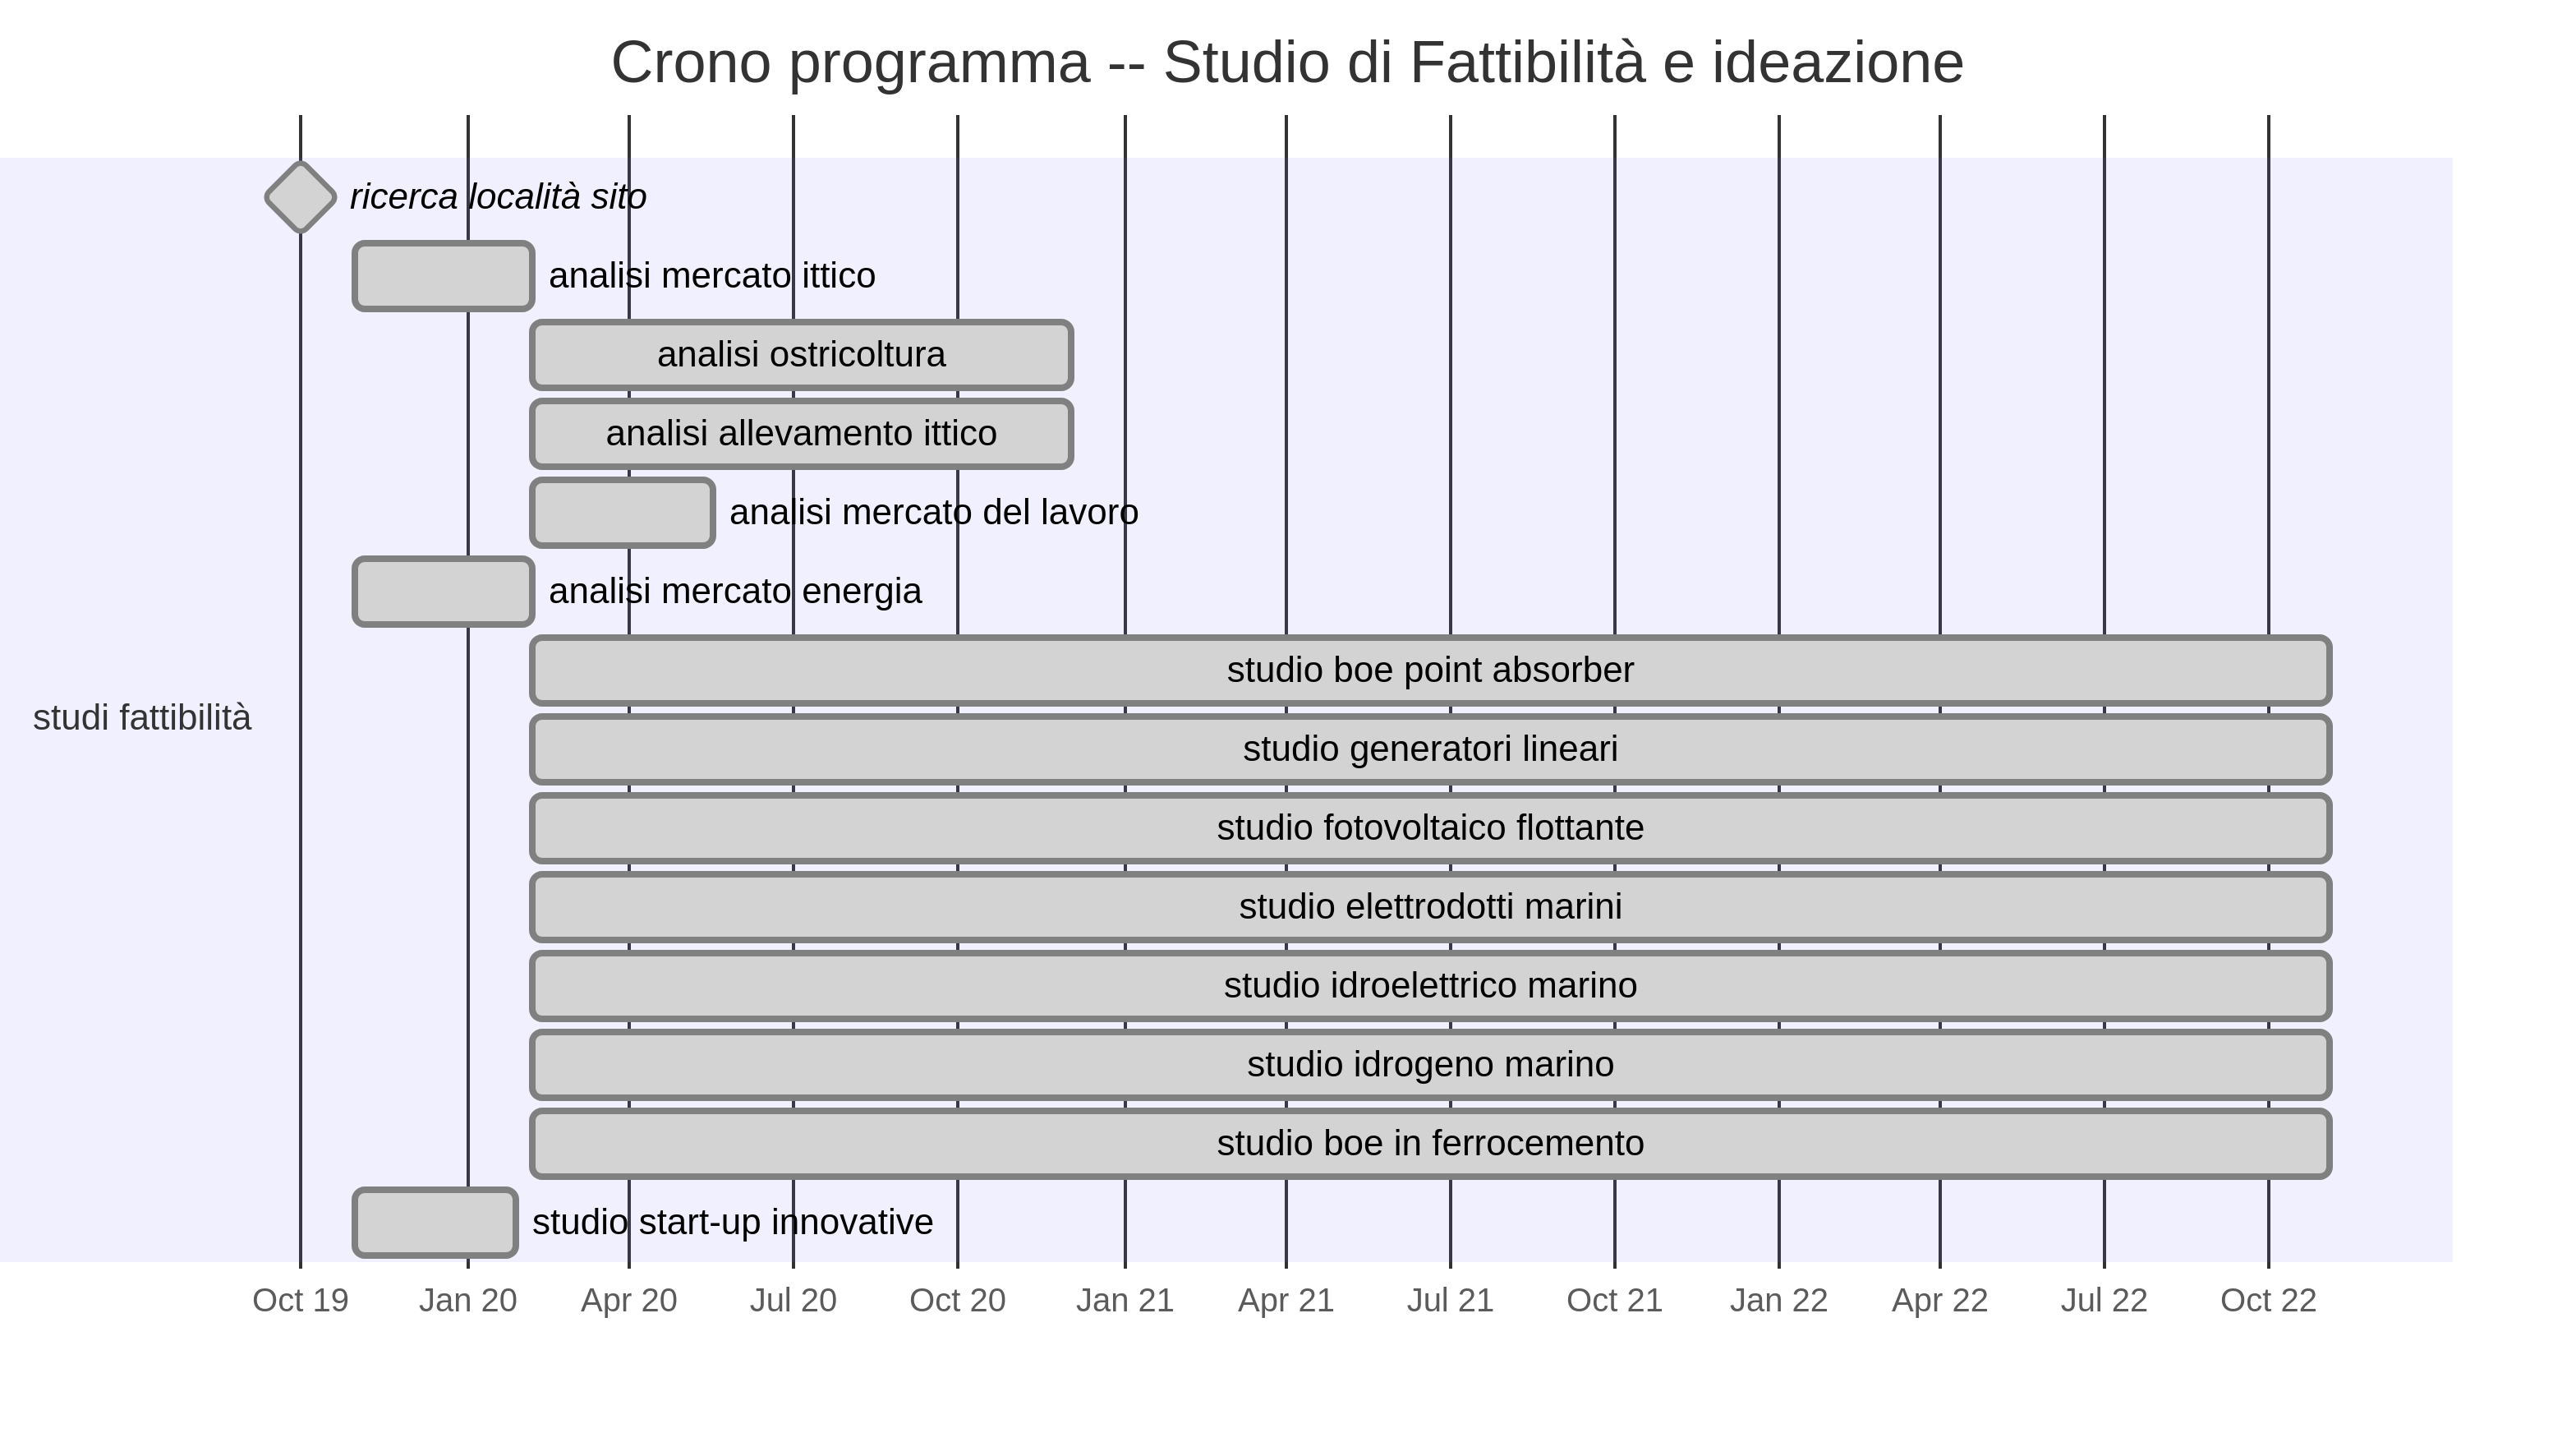
\includegraphics[width=8.17in,height=4.54in]{lettera_files/figure-latex/mermaid-figure-1.png}

}

\end{figure}

\begin{figure}[H]

{\centering 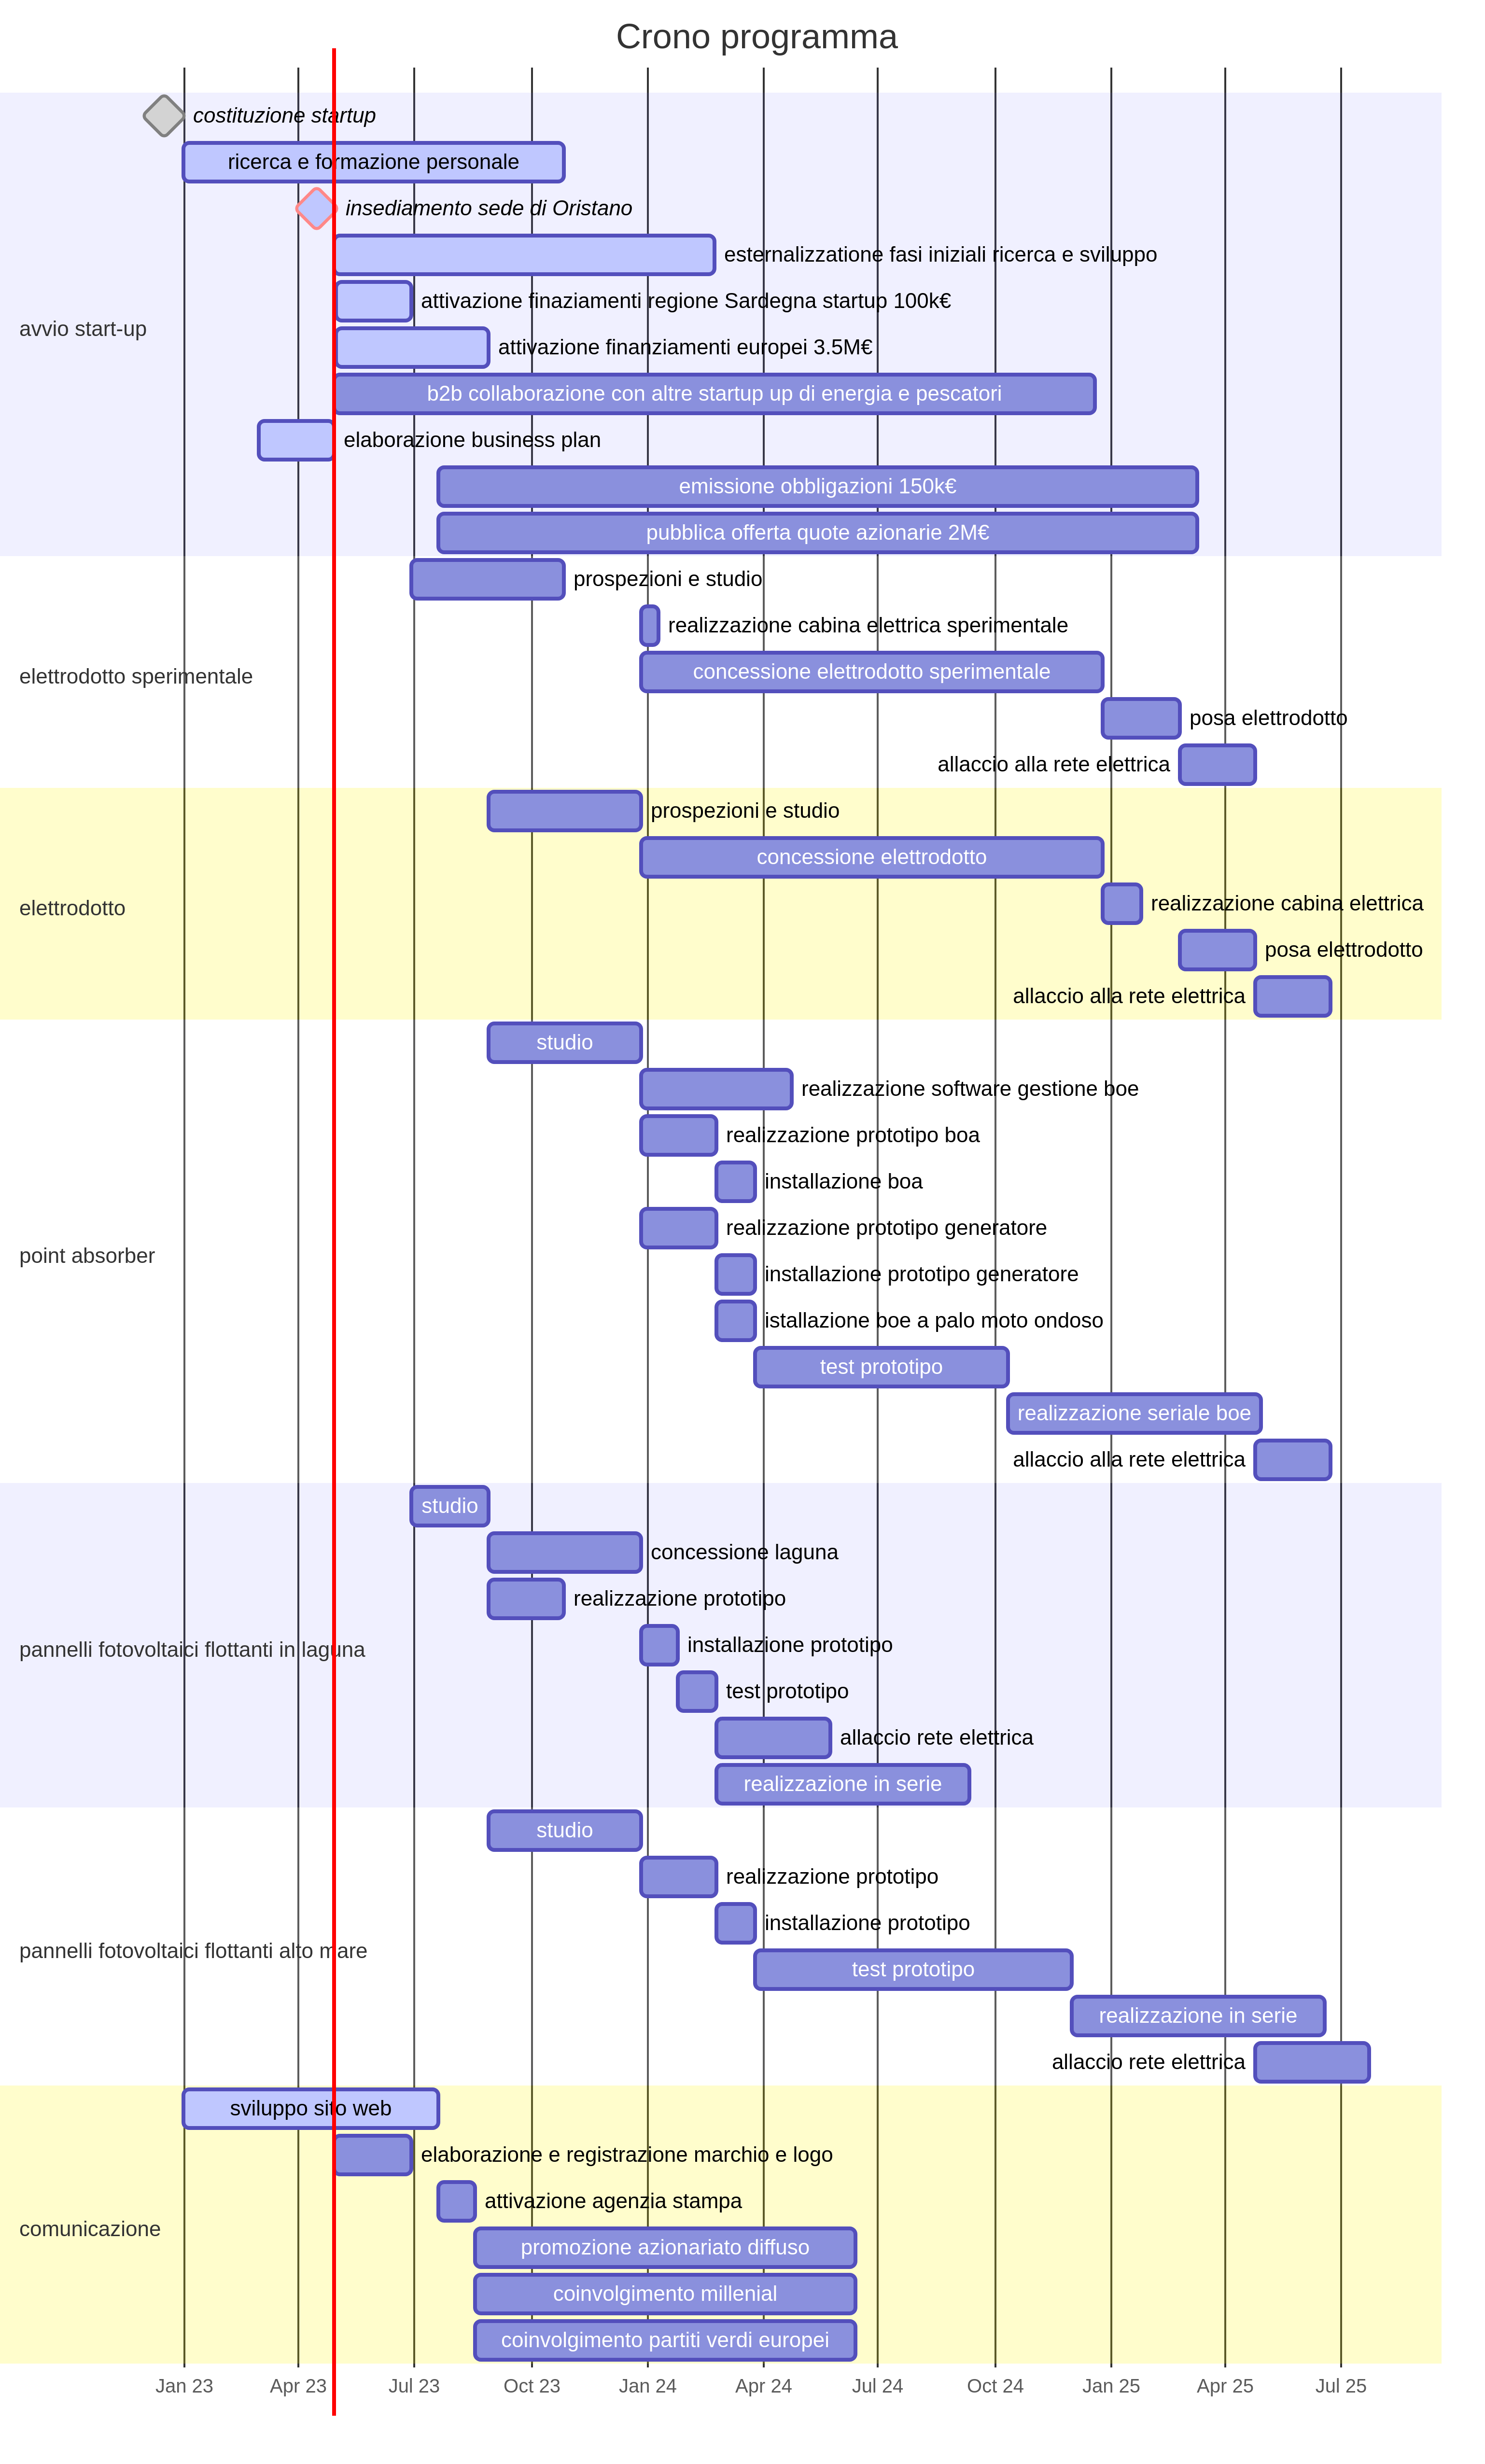
\includegraphics[width=8.17in,height=13.29in]{lettera_files/figure-latex/mermaid-figure-2.png}

}

\end{figure}



\end{document}
